\section{使用通用引用的重载}
已经讨论了将对象绑定到普通引用时的规则。现在,在引入通用引用之后,必须扩展这些规则。

再次假设有一个类X,有一个非\cppinline{const}变量\cppinline{v},有一个\cppinline{const}变量\cppinline{c}:

\begin{cppcode}
class X {
	...
};

X v;
const X c{ ... };
\end{cppcode}

如果提供函数\cppinline{f()}的所有重载,根据正式规则,就是下面列出所有重载:

\begin{cppcode}
void f(const X&); // read-only access
void f(X&); // OUT parameter (usually long-living object)
void f(X&&); // can steal value (object usually about to die)
void f(const X&&); // contradicting semantic meaning
template<typename T>
void f(T&&); // to use perfect forwarding
\end{cppcode}

\subsubsection{表 9.1. 绑定所有引用规则}
\begin{center}
	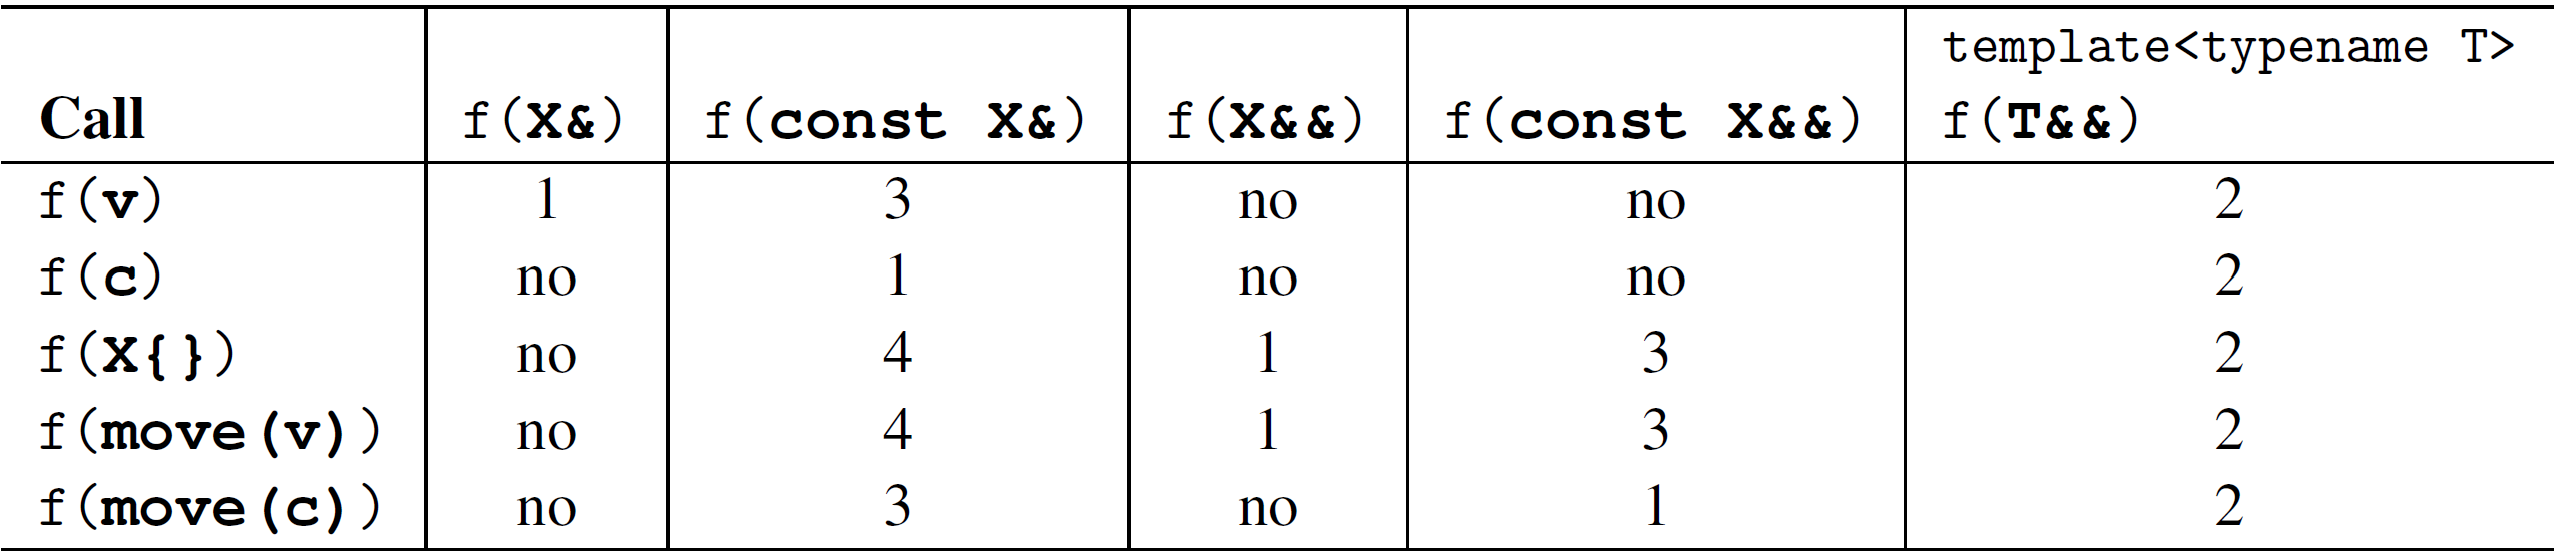
\includegraphics[width=0.8\textwidth]{part2/ch9/images/1}
\end{center}

同样,这些数字列出了重载解析的优先级(最小的数字具有最高的优先级),以便确定重载时调用了哪个函数。

请注意,通用引用总是次优选择。完美匹配总是优先,但是需要转换类型(例如使其为\cppinline{const}或将rvalue转换为lvalue)是比为精确类型实例化函数模板更糟糕的匹配方式。

\subsection{用通用引用修正重载解析}

重载解析中,通用引用绑定比类型转换更好,这有一个非常糟糕的副作用:如果有一个接受单个通用引用的构造函数,那么这个匹配就要比以下方式更优

\begin{itemize}
	\item 如果传递非\cppinline{const}对象,则使用复制构造函数
	\item 如果传递\cppinline{const}对象,则使用移动构造函数
\end{itemize}

因此,实现只有一个通用引用参数的构造函数时,必须谨慎。

思考下面的代码:

\filename{generic/universalconstructor.cpp}
\begin{cppcode}
#include <iostream>

class X {
public:
	X() = default;
	X(const X&) {
		std::cout << "copy constructor\n";
	}
	X(X&&) {
		std::cout << "move constructor\n";
	}

	template<typename T>
	X(T&&) {
		std::cout << "universal constructor\n";
	}
};
int main()
{
	X xv;
	const X xc;

	X xcc{xc}; // OK: calls copy constructor
	X xvc{xv}; // OOPS: calls universal constructor
	X xvm{std::move(xv)}; // OK: calls move constructor
	X xcm{std::move(xc)}; // OOPS: calls universal constructor
}
\end{cppcode}

如注释中所示,该程序有以下输出:

\begin{outputcode}
copy constructor
universal constructor
move constructor
universal constructor
\end{outputcode}

因此,最好避免实现将第一个形参声明为通用引用,并为任意类型的实参调用的泛型构造函数。

另一种选择是,传递的是类的类型(或可转换为),则以禁用构造函数的方式约束构造函数。其必须使用在复制或移动构造函数上才有效果。从C++20起,可以写成这样:

\begin{cppcode}
class X {
	public:
	...
	template<typename T>
	requires (!std::is_same_v<std::remove_cvref_t<T>, X>)
	X(T&&) {
		std::cout << "universal constructor\n";
	}
};
\end{cppcode}

C++20前,需要这样写:

\begin{cppcode}
class X {
	public:
	...
	template<typename T,
	typename
	= typename std::enable_if<!std::is_same<typename std::decay<T>::type,
	X>::value
	>::type>
	X(T&&) {
		std::cout << "universal constructor\n";
	}
};
\end{cppcode}


















